\documentclass[aspectratio=169]{beamer}

\usepackage{algo}
\usepackage{sigmastyle}
\usepackage{mathdots}

\setbeamertemplate{blocks}[rounded]
\usecolortheme{orchid}
\usetheme{sigma}

\title{Dynamics and Chaos: the Logistic Map}
\author{Hanyang Sha}
\date{03-31-2025}

\begin{document}

\begin{frame}
\titlepage
\end{frame}

\begin{frame}{Contents}
\tableofcontents
\end{frame}

\section{Introduction: $0<\mu<3$}
\frame{\sectionpage}

\begin{frame}{Definition}
    A 1D map can be expressed in the form of $x_{n+1} = f(x_n)$. 
    \begin{defn}
        The \textbf{logistic map} is a family of functions $f\mu: \mathbb{R}\rightarrow \mathbb{R}, x \mapsto \mu x(1-x),\mu\in\mathbb{R}$.
    \end{defn}
    Specifically, we will investigate $\mu>0$.
\end{frame}

\begin{frame}{Immediate Observations}
\begin{itemize}
    \item Recall that fixed point $x_*$ is \textbf{stable/attracting} if $\lvert f'(x_*) \rvert < 1$ and \textbf{unstable/repelling} if $\lvert f'(x_*) \rvert > 1$. Bifurcations usually occur at the \textbf{marginally stable} point of $\lvert f'(x_*) \rvert = 1$. 
    \item The initial fixed points for small $\mu$ are: $x = \mu x(1-x) \rightarrow x_* = 0, 1-1/\mu$. $f'_\mu = \mu(1-2x)$, so $x_* = 0$ is stable for $0 < \mu < 1$, and $x_* = 1-1/\mu$ is stable for $1 < \mu < 3$.
\end{itemize}
\end{frame}

\begin{frame}{The $1<\mu<3$ Case}
\begin{prop}
    Suppose $\mu> 1$. If $x < 0$ or $x > 1$, then $\displaystyle\lim_{n\rightarrow\infty} f_\mu^n(x) = -\infty$. 
\end{prop}
\begin{pf}
    Note that if $x>1$, $f_\mu(x) = \mu x(1-x) < 0$, reducing to the $x<0$ case. Note that $x > f_\mu(x)$, so $(f_\mu^n(x))_n$ forms a decreasing sequence. We now show that this sequence cannot converge. Suppose for some $x<0$, $f_\mu^n(x)\rightarrow p$ for some $p$. Then $f_\mu^{n+1}(x) \rightarrow p$. But by continuity of $f$, $f_\mu^{n+1}(x) \rightarrow f_\mu(p) < p$. Contradiction. 
\end{pf}
\end{frame}

\begin{frame}{The $1<\mu<3$ Case (cont.)}
\begin{prop}
    If $0<x<1$, then $\displaystyle \lim_{n\rightarrow\infty} f_\mu^n(x) = x_*$, where $x_* = 1-1/\mu$ (as expected, because $x_*$ is an attracting fixed point. 
\end{prop}
\begin{pf}[draw a picture]
    We split into 3 cases: $1<\mu<2$, $\mu =2$, $2 <\mu<3$. One can check for the second case explicitly. 
    For $1<\mu<2$, $x_* < 1/2$, and $f_\mu(x)<x$ for $0<x<1/2$. Thus, for $0<x<x_*$, $f_\mu(x) > x$, and $(f_\mu^n(x))_n$ converges to $x_*$. Similarly, for $x_* < x < 1/2$, $f_\mu(x) < x$, and $(f_\mu^n(x))_n$ converges to $x_*$. Note $f((1/2,1)) = (0,1/2)$, and $1/2<x<1$ is proved as well. 
    For $2<\mu<3$, $x_* > 1/2$. Define $x_*' = 1/\mu$ (reflecting $x_*$ across $x=1/2$). For $0<x<x_*'$, $f_\mu(x) > x$. For $x_*'<x<x_*$, although $f_\mu(x)>x_*$, note that $x< f_\mu^2(x) < x_*$ (can be shown by taking derivative). Thus, we have proved for $0<x<x_*$. For $x_*<x<1$, note that $f((x_*,1))=(0,x_*)$, hence proved. 
\end{pf}
\end{frame}

\begin{frame}{The $0<\mu<1$ Case}
\begin{itemize}
    \item We have similar results. 
    \item Now $x_*=1-1/\mu<0$. 
    \item Specifically, for $x<x_*$ or $x>1/\mu$, $\displaystyle\lim_{n\rightarrow \infty} f_\mu^n(x) = -\infty$, and for $x_* < x < 1/\mu$, $\displaystyle\lim_{n\rightarrow \infty} f_\mu^n(x) = 0$, as expected, because 0 is an attracting fixed point. 
\end{itemize}
\end{frame}

\begin{frame}{For $\mu>3$...}
\begin{itemize}
    \item Period doubling for $\mu < 3.56995$.  
    \item Most values of $\mu \in (3.56995,4)$ exhibit chaotic behavior, but there are still certain isolated ranges of $\mu$ that show non-chaotic behavior; these are sometimes called islands of stability (Wikipedia).
    \item All $\mu > 4$ exhibit chaotic behavior. 
\end{itemize}
\end{frame}

\section{Bifurcations: $3<\mu< \mu_\infty$}
\frame{\sectionpage}

\begin{frame}{Bifurcation}
\begin{itemize}
    \item Let $\lambda$ be a external parameter. Let $f:X\rightarrow X$ be a function dependent on $\lambda$. Varying $\lambda$ generates a family of functions, denoted $f_\lambda$, where each function in the family uses a different value of $\lambda$. 
    \item As we change $f$ by varying $\lambda$, there are certain points in the family where the qualitative behavior of the function changes. These changes are called \textbf{bifurcations}, and the values of the parameter $\lambda$ where these changes occur are called \textbf{bifurcation points}.
\end{itemize}
\end{frame}

\begin{frame}{Period Doubling Bifurcation: Definition}
\begin{defn}
    A family of functions $f_\lambda$ undergoes a \textbf{period doubling bifurcation} at $\lambda = \lambda_0$ if $\exists$ open interval $I$, $\epsilon >0$ s.t.: 
    \begin{enumerate}
        \item $\forall \lambda \in [\lambda_0-\epsilon, \lambda_0+\epsilon], \exists !$ fixed point $p_\lambda \in I$ for $f_\lambda$.
        \item $\forall \lambda \in (\lambda_0-\epsilon, \lambda_0], f_\lambda$ has no cycles of period 2 in $I$ and $p_\lambda$ is attracting (resp. repelling). 
        \item $\forall \lambda \in (\lambda_0, \lambda_0+\epsilon), \exists !$ 2-cycle $q_\lambda^1, q_\lambda^2$ in $I$ that is attracting (resp. repelling). Meantime, fixed point $p_\lambda$ is repelling (resp. attracting). 
        \item As $\lambda\rightarrow\lambda_0$, $q_\lambda^i \rightarrow p_{\lambda_0}$.
    \end{enumerate}
\end{defn}
\end{frame}

\begin{frame}{First Period Doubling Bifurcation}
\begin{itemize}
    \item At $\mu = 3$, $x_* = 1-1/3 = 2/3$, and $f'_\mu(x_*) = \mu(1-2x_*) = 3(1-2 \cdot 2/3) = -1$, which is a marginally stable point, causing the first bifurcation.
    \item The 2 periodic points (denoted $x_0$ and $x_1$) after the bifurcation must both satisfy $x = f_\mu(f_\mu(x)) = f_\mu^2(x)$, which is a quartic equation. Note that 2 roots are the initial fixed points $x_* = 0, 1-1/\mu$, so factor them out to get $ x_1, x_2 = \frac{1}{2\mu}(\mu+1 \pm \sqrt{(\mu+1)(\mu-3)})$.
\end{itemize}
\end{frame}

\begin{frame}{Subsequent Period Doubling Bifurcations}
\begin{itemize}
    \item To find the value of $\mu$ at which a bifurcation occurs (going from period-$2^{n-1}$ to period-$2^n$, we use $(f_\mu^{2^{n-1}})'(x_i) = -1$ for all fixed points $x_i$ of $f_\mu^{2^{n-1}}$. 
    \item Using the chain rule, $(f_\mu^{2^{n-1}})'(x_0) = f'_\mu(f^{2^{n-1}-1}_\mu(x_0))f'_\mu(f^{2^{n-1}-2}_\mu(x_0)) \cdots f'_\mu(f_\mu(x_0)) f'_\mu(x_0)$ $= f'_\mu(x_{2^{n-1}-1}) f'_\mu(x_{2^{n-2}-2}) \cdots f'_\mu(x_1) f'_\mu(x_0) = \displaystyle \prod_{i=0}^{2^{n-1}-1} f'_\mu(x_i) = \displaystyle \prod_{i=0}^{2^{n-1}-1} \mu(1-2x_i) = -1.$
    \item We know where the fixed points $x_i$ are for period-$2^{n-1}$, so we can solve the equation as a function in $\mu$.
\end{itemize}
\end{frame}

\begin{frame}{Feigenbaum Constant}
\begin{itemize}
    \item It turns out that if we take the ratio of the space between consecutive period doubling bifurcation points of the logistic map, we approach a value known as the Feigenbaum constant $\delta \approx 4.669...$ (A006890 in OEIS). 
    \item Let $q_n$ be the value of $q$ of the $n$-th bifurcation. Let $\delta_n := \frac{q_{n+1} - q_n}{q_{n+2} - q_{n+1}}$. Then $\delta := \displaystyle \lim_{n \rightarrow \infty} \delta_n$. 
    \item As expected from geometric series, $q_n$ converges. We denote the limit as $\mu_\infty \approx 3.56994...$ (A098587 in OEIS). 
    \item This constant is \textit{universal} for all 1D maps with a single locally quadratic maximum. 
\end{itemize}
\end{frame}

\begin{frame}{Renormalization}
\begin{figure}[htp]
    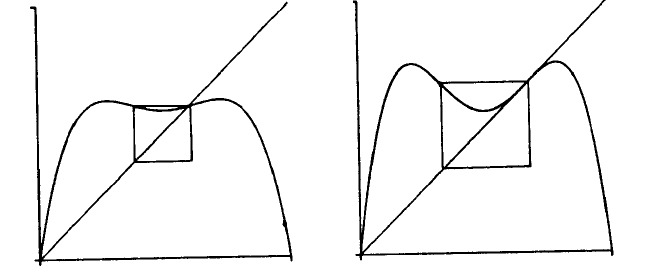
\includegraphics[width=6cm]{images/renorm1.png}
    \label{fig:renorm1}
\end{figure}
\begin{figure}[htp]
    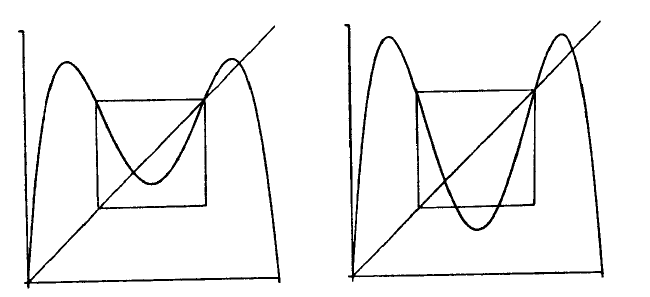
\includegraphics[width=6cm]{images/renorm2.png}
    \label{fig:renorm2}
    \caption{$f_\mu^2(x)$ for increasing $\mu$, $2<\mu<4.$}
\end{figure}
\end{frame}

\begin{frame}{Renormalization (cont.)}
\begin{defn}
    Let $p_\mu$ be the periodic point of period 2 of $f_\mu$, and let $p_\mu^*$ be the point s.t. $f(p_\mu^*) = p_\mu$. $L_\mu(x) := \frac{1}{p_\mu^*-p_\mu}(x-p_\mu)$. The \textbf{renormalization} of $f_\mu$ is defined as $(Rf_\mu)(x) := L_\mu\circ f_\mu^2 \circ L^{-1}(x)$. 
\end{defn}
\begin{itemize}
    \item $Rf_\mu$ provides a magnified view of the local behavior.  
    \item Observation: if $x$ is a periodic point of period 2 of $f_\mu$, then $L(x)$ is a fixed point of $(Rf_\mu)(x)$.
    \item Repeated renormalization leads to a sequence of bifurcation points that we expected. 
\end{itemize}
 
\end{frame}

\section{Symbolic Dynamics}
\frame{\sectionpage}

\begin{frame}{An Alternative Metric Space}
\begin{defn}
    Let $\Sigma_2 := \{s = (s_0s_1\cdots) : s_j=0 \text{ or } 1 \forall j\}$ be the set of all bitstrings of infinite length. Let $\forall s,t \in \Sigma_2, d(s,t) := \displaystyle\sum_{i=0}^\infty \frac{|s_i-t_i|}{2^i}$. 
\end{defn}
\begin{prop}
    $d$ is a metric on $\Sigma_2$. 
\end{prop}
Observation: $s,t \in \Sigma_2$. If $s_i=t_i \forall i, 0\leq i\leq n$, then $d(s,t)\leq 2^{-n}$. If $d(s,t)< 2^{-n}$, then $s_i=t_i \forall i, 0\leq i\leq n$. 
\end{frame}

\begin{frame}{The Shift Map $\sigma$}
\begin{defn}
    $\sigma: \Sigma_2 \rightarrow \Sigma_2, \sigma(s_0s_1s_2\cdots) = (s_1s_2s_3\cdots)$. 
\end{defn}
\begin{prop}
    $\sigma$ continuous. 
\end{prop}
\end{frame}

\begin{frame}{Properties of $\sigma$}
\begin{prop}
\begin{enumerate}
    \item Number of periodic points of period $n$ is $2^n$. 
    \item Periodic points are dense in $\Sigma_2$. 
    \item There exists dense orbit in $\Sigma_2$. 
\end{enumerate}
\end{prop}
\begin{cor}
    $\sigma$ is chaotic in $\Sigma_2$. 
\end{cor}
\end{frame}

\begin{frame}{Proof of Proposition}
\begin{pf}
\begin{enumerate}
    \item A periodic point of period $n$ is in the form of $s_0\cdots s_{n-1}s_0\cdots s_{n-1}\cdots$, so there are $2^n$ such periodic points. 
    \item We want $\forall t\in \Sigma_2, \epsilon>0 \exists$ periodic point $s : d(s,t)<\epsilon$. Note $\exists M: s_i=t_i \forall 0\leq i\leq M \rightarrow d(s,t)<\epsilon$. Take $s = (t_0\cdots t_Mt_0\cdots t_M\cdots)$. 
    \item We want $\exists s\in\Sigma_2 : \forall t\in \Sigma_2, \epsilon>0 \exists N: d(\sigma^N(s),t) <\epsilon$. Note again $\forall\epsilon \exists M: \sigma^N(s)=t_i \forall 0\leq i\leq M \rightarrow d(\sigma^N(s),t)<\epsilon$. Denote $s_M$ to be a concatenation of an enumeration of all bitstrings of length $M$. Take $s=$ concatenation of all $s_M \forall M\in \mathbb{N}$. 
\end{enumerate}
\end{pf}
\end{frame}

\section{Topological Conjugacy: $\mu>4$}
\frame{\sectionpage}

\begin{frame}{The Set $\Lambda$}
\begin{defn}
    Let $A_n = \{x \in [0,1]: f_\mu^n(x) \in [0,1],f_\mu^{n+1}(x) \notin [0,1]\}.$ Define $\Lambda := [0,1]-\displaystyle\bigcup_{n=0}^\infty A_n$.  
\end{defn}
\begin{defn}
    A set $S$ is a \textbf{Cantor set} if it is closed, totally disconnected (contains no intervals as connected subsets), and perfect (every point in $S$ is an accumulation point of all other points in $S$). 
\end{defn}
\begin{prop}
    $\Lambda$ is a Cantor set for $\mu>4$. 
\end{prop}
\end{frame}

\begin{frame}{Proof of Cantor-ness}
\begin{pf}
\begin{itemize}
    \item Closed: we start with a closed interval. At every iteration, an open interval is removed (equivalent of taking the intersection with a closed interval). Intersection of closed intervals are closed. 
    \item Totally disconnected: we shall see this shortly. 
    \item Perfect: suppose not. Then there exists isolated point $p \in\Lambda$. Then exists some $i$ s.t. $\forall x\in \overline{B_\epsilon^o}(p), f_\mu^i(x)<0$. Thus, $f_\mu^i$ is maximized at $p$, so $(f_\mu^i)'(p)=0$. This implies that $f'(f_\mu^j(p))=0$ for some $j<i$. But this means $f_\mu^j(p) = 1/2$, which is a contradiction because $f_\mu^{j+1}(p) \notin \Lambda$.   
\end{itemize}
\end{pf}
\end{frame}

\begin{frame}{Definitions}
\begin{defn}
    A function $f:X\rightarrow Y$ between two spaces $X,Y$ is a \textbf{homeomorphism} if
    \begin{enumerate}
        \item is a bijection
        \item is continuous 
        \item has continuous inverse
    \end{enumerate}
\end{defn}
\begin{defn}
    Let $f:X\rightarrow X$, $g:Y\rightarrow Y$. Then $f,g$ are \textbf{topologically conjugate} if there exists homeomorphism $h:X\rightarrow Y$ s.t. $h\circ f = g\circ h$. 
\end{defn}
\end{frame}

\begin{frame}{A Preliminary Theorem}
\begin{defn}
    Let $S: \Lambda \rightarrow \Sigma_2$ be the following function: $x\in\Lambda, S(x)=s_0s_1\cdots$, where $s_i=0$ if $f_\mu^i(x) \in I_0$ and $s_i=1$ if $f_\mu^i(x) \in I_1$, where $I_0 = \{x \in [0,1/2] : f_\mu(x)\leq 1\}$ and $I_1 = \{x \in [1/2,1] : f_\mu(x)\leq 1\}$. 
\end{defn}
\begin{thrm}
    If $\mu>2+\sqrt5$, then $S:\Lambda \rightarrow \Sigma_2$ is a homeomorphism. 
\end{thrm}
\end{frame}

\begin{frame}{Continuity of $S$}
\begin{pf}
    We will use the sequential criterion of continuity. Consider arbitrary sequence $(x_n) \subset \Lambda$ with $x_n \rightarrow x \in \Lambda$. We want $S(x_n) \rightarrow S(x) \in \Sigma_2$, i.e., $\forall \epsilon>0, \exists N: n>N \rightarrow d(S(x_n),S(x)) < \epsilon$. Note that $d(S(x_n),S(x)) < \epsilon \leftrightarrow \exists M : (S(x_n))_i = (S(x))_i \forall i\leq M$ (take $M$ s.t. $2^{-M} < \epsilon$). This means that $\forall i \leq M$, $f_\mu^i(x_n)$ and $f_\mu^i(x)$ agree on whether they are in $I_0$ or $I_1$. 
    Let $J_i$ be the interval (either $I_0$ or $I_1$) that $f_\mu^i(x)$ is in. For each $i, 0\leq i \leq M$, let us pick $\epsilon_i>0, \epsilon_i \leq |f_\mu^i(x_n)-f_\mu^i(x)|,$ s.t. $\forall y: |y-f_\mu^i(x)| < \epsilon_i,y \in J_i$. Note that $f_\mu^i$ continuous everywhere $\forall i$. Thus, $\exists \delta_i>0 : |y-x| < \delta_i \rightarrow |f_\mu^i(y)-f_\mu^i(x)| < \epsilon_i$. Take $\delta := \displaystyle\min_{0\leq i\leq M} \delta_i$. Because $x_n \rightarrow x$, $\exists N: n>N \rightarrow |x_n-x| < \delta$. Take this $N$. $\blacksquare$ 
\end{pf}
\end{frame}

\begin{frame}{Continuity of $S^{-1}$}
\begin{pf}
    We again use the sequential criterion of continuity. Consider arbitrary sequence $(y_n) \subset \Sigma_2$ with $y_n \rightarrow y \in \Sigma_2$. Define $x_i := S^{-1}(y_i) \in \Lambda \forall i$ and $x := S^{-1}(y)$; we want $x_i \rightarrow x$. Suppose not. Then there exists $\epsilon>0$ and subsequence $(x_{n_k})_k \subset (x_n)_n$ s.t. $\forall k, |x_{n_k}-x|\geq \epsilon$. Observe that $\mu>2+\sqrt5 \rightarrow |f_\mu'(x)|>1 \forall x \in I_0 \cup I_1$. Then by MVT, $|f_\mu(x_{n_k})-f_\mu(x)| > \lambda|x_{n_k}-x|$, for some $\lambda>1$. This implies $|f_\mu^i(x_{n_k})-f_\mu^i(x)| > \lambda^i|x_{n_k}-x| \geq \lambda^i\epsilon$, which is unbounded. Note that $y_n \rightarrow y$ means that $\forall M\in \mathbb{N}, \exists N: n>N \rightarrow$  $\forall 0\leq i \leq M$, $f_\mu^i(x_n)$ and $f_\mu^i(x)$ agree on whether they are in $I_0$ or $I_1$. But this is a contradiction, because for large enough $M$, $\forall N\exists n>N$ s.t. $|f_\mu^M(x_n)-f_\mu^M(x)| > len(I_0) = len(I_1)$. $\blacksquare$ 
\end{pf}
\end{frame}

\begin{frame}{Alternative Proof for $S^{-1}$}
\begin{pf}
    Note that $\Lambda$ compact. By the Heine-Borel theorem, boundedness and totally boundedness are equivalent on $\mathbb{R}^n$. Obviously, $\Lambda$ is closed and bounded. Recall that compact is equivalent to closed AND totally bounded.  \\
    Recall from topology that a continuous bijection with compact domain has continuous inverse. Done! 
\end{pf}
\end{frame}

\begin{frame}{Bijection}
\begin{pf}
    Injectivity: Suppose $S(x)=S(y)$ for $x,y\in \Lambda$. Then $\forall n\in\mathbb{N}$, $f_\mu^n(x)$ and $f_\mu^n(y)$ agree on whether they are in $I_0$ or $I_1$. Suppose $x\neq y$. Then similar the previous proof, we have $|f_\mu^n(x_{n_k})-f_\mu^n(x)| > \lambda^n|x_{n_k}-x| \geq \lambda^n\epsilon$. Contradiction. \\
    Surjectivity: Define $I_{s_0s_1\cdots s_n} = \{x \in\Lambda: x\in I_{s_0}, f_\mu(x)\in I_{s_1}, \cdots, f_\mu^n(x)\in I_{s_n}\} = I_{s_0} \cap f_\mu^{-1}(I_{s_1s_2\cdots s_n})$. By induction, $I_{s_1s_2\cdots s_n}$ is closed and nonempty. By continuity of $f$, $f_\mu^{-1}(I_{s_1s_2\cdots s_n})$ is closed. Note that $I_{s_0}$ closed, so because intersection of closed sets is closed, $I_{s_0s_1\cdots s_n}$ closed. Note that $f_\mu^{-1}(I_{s_1s_2\cdots s_n}) = I_{0s_1s_2\cdots s_n}\cup I_{0s_1s_2\cdots s_n}$, both of which are nonempty, so $I_{s_0s_1\cdots s_n}$ nonempty. Consider arbitrary $y\in\Sigma_2, S(y)=(s_0s_1\cdots)$, we have $\displaystyle\bigcap_{n=0}^\infty I_{s_0\cdots s_n}$ is closed. Moreover, we know that it only contains 1 element: $f_\mu^{-1}(y)$. $\blacksquare$
\end{pf}
\end{frame}

\begin{frame}{Topological Conjugacy}
\begin{thrm}
    $S \circ f = \sigma\circ S$. 
\end{thrm}
\begin{pf}
    We will show $f = S^{-1}\circ\sigma\circ S$. Suppose $x\in\Lambda$, $S(x)=(s_0s_1\cdots)$. Then $S^{-1}\circ\sigma\circ S(x) = S^{-1}(s_1\cdots) = \displaystyle\bigcap_{n=1}^\infty I_{s_1\cdots s_n}$, which is obviously equal to $f(x)$. 
\end{pf}
\end{frame}

\begin{frame}{$S$ as Topological Conjugate}
\begin{itemize}
    \item Due to the topological conjugacy between $\Lambda$ and $\Sigma_2$ via $S$, all dynamics properties on the two spaces area equivalent. 
    \item Specifically, we have periodic points are dense in $\Lambda$, and there exists dense orbit in $\Lambda$. 
    \item Thus, we have $f_\mu$ chaotic in $\Lambda$ for $\mu>2+\sqrt5$.
    \item This is actually true for $\mu>4$, by first taking a homeomorphism between the logistic map and the tent map, then proving chaos for the tent map using a topological conjugacy between the tent map and $\Sigma_2$. 
\end{itemize}
\end{frame}

\begin{frame}{}
      \begin{center}
    {\color{sigma@mainblue} \LARGE Questions?}
  \end{center}
\end{frame}

\begin{frame}[allowframebreaks]{Bibliography}
    \tiny
    \bibliography{refs}
    \bibliographystyle{alpha}
    \begin{itemize}
        \item Devaney, Robert (1989). \textit{A First Course in Chaotic Dynamical Systems}. CRC Press.
        \item Devaney, Robert (1989). \textit{An Introduction to Chaotic Dynamical Systems}. Addison-Wesley.
        \item Teschl, Gerald (2007). \textit{Ordinary Differential Equations and Dynamical Systems}. American Mathematical Society. 
    \end{itemize}
\end{frame}

\end{document}